\section{Preliminaries}\label{sec:preliminaries}

Here i present all relevant terminology, notation and definitions that will be used throughout the report. Be aware that my notation does not use the most common notations from the literature, but instead uses a notation that i find more intuitive, which mostly means that use different letters than other literature, in order to better distinguish between the different types of goods.

% Just keep this here in case something changes later
\def\sGood{g}
\def\sAllGoods{G}
\def\sNumGoods{m}

\def\sItem{i}
\def\sAllItems{I}
\def\sNumItems{i_n}

\def\sCake{c}
\def\sTheCake{C}
\def\sAllCakes{C}
\def\sNumCakes{c_n}

\def\sAgent{a}
\def\sAllAgents{A}
\def\sNumAgents{n}

\def\sValuation{v}
\def\sAllValuations{V}
\def\sNumValuations{v_n}

\def\sAllocation{\scalebox{1.25}{$\mathpzc{A}$}}
\def\sInstance{\scalebox{1.1}{I}}
\def\sBundle{B}

\def\MMS{\text{MMS}}
\def\halfMMS{\frac{1}{2}\text{MMS}}
\def\PROP{\text{PROP}}
\def\R{\mathbb{R}}


\subsection*{Mixed Goods}
When discussion mixed goods we are talking about a mix of both indivisible (i.e. paintings, cars etc.) and divisible goods (i.e. money, land, fuel, time etc.) . A mixed goods instance can contain any combination of number of divisible and indivisible goods.

\textbf{Item}\\
An indivisible good will be referred to as an \emph{item}, $\sItem$, where the number of items $\sNumItems$ defines the set of all items $\sAllItems$. Formally:
$$\sItem\in\{1,2,...,\sNumItems\}\equiv\sItem\in\sAllItems$$

\textbf{Cake}\\
A divisible good will be referred to as \emph{cake}, $\sCake$, where the number of cakes $\sNumCakes$ defines the set of all cakes $\sAllCakes$. Formally:
$$\sCake\in\{\sCake_1, \sCake_2, ...,\sNumCakes\}\equiv\sCake\in\sAllCakes$$
Furthermore, since a cake is divisible, a piece of the cake will be defined as en interval of the entire cake, where the entire cake is defined over the interval $[0,1]$, such that $\sCake=\sCake_{[0,1]}$.
A slice of the cake is then defined as $\sCake_{[x,y]}$ where $x,y \in [0,1]$ and $x \leq y$ where the size of the slices of cake is $\sCake_y-\sCake_x$. As this project focuses on homogenous cake (see \autoref{subsec:homogenous-cake}), the exact interval of the cake is not important, a slice of cake will for this project then only needs to be specified to by its size $z$, where $\sCake_z\equiv\sCake_y-\sCake_x\equiv\sCake_{[x,y]}$ where we can assume $x=0$.

\textbf{Good}\\
Since we are in a mixed setting, a good can be either divisible or indivisible. It is therefor convenient to able to refer to goods $\sGood$ that can be either an item or cake. Formally:
$$\sGood\in\{1,2,...,\sNumItems\}\cup\{\sCake_1, \sCake_2, ...,\sNumCakes\}\equiv\sGood\in\sAllItems\cup\sAllCakes\equiv\sGood\in\sAllGoods$$



\subsection*{Homogenous Cake}\label{subsec:homogenous-cake}
A \emph{Homogenous cake} is a cake where all agents valuations for a piece of cake is only proportional to the size of the piece of cake. Formally, for a piece of cake from $x$ to $y$ ($\sCake_{[x,y]}$) and an agent $\sAgent\in\sAllAgents$ the value of the pieces is proportional to that agents value of the entire cake:
$$\sValuation_\sAgent(\sCake_{[x,y]})=(y-x)\sValuation_\sAgent(\sCake)$$



\subsection*{Heterogenous Cake}
A \emph{Heterogenous Cake} is a cake in which each agent has their own density function $d_\sAgent:[0,1]\rightarrow\R^+\cup\{0\}$ which captures how the agent values different parts of the cake. The value of agent $\sAgent$ over a finite union of intervals $S \subseteq [0, 1]$ is defined as $\sValuation_\sAgent(S) = \int_S d_\sAgent dx$.



\subsection*{Agent}
An agent $\sAgent$ is a person or entity that is to be allocated goods. The number of agents $\sNumAgents$ defines the set of all agents $\sAllAgents$. Formally:
$$\sAgent\in\{1,2,...,\sNumAgents\}\equiv\sAgent\in\sAllAgents$$



\subsection*{Valuations}
A valuation $\sValuation_\sAgent$ is a function for each agent $\sAgent$ that takes a set of goods $\{\sGood_1, \sGood_2,...\}$ and finds this agents value for this set of goods. For simplicity we will write $\sValuation_\sAgent(\{\sGood\})$ as $\sValuation_\sAgent(\sGood)$. Since we only are dealing with goods, we have that the value for all items for all agents is positive, formally:
$$\forall\sAgent\in\sAllAgents, \forall\sGood\in\sAllGoods, \sValuation_\sAgent(\sGood)\geq0$$



\subsection*{Additive valuations}
A well-studied subclass of monotone valuations is that of additive valuations, where an agent's value of any subset of items is equal to the sum of the values of individual items in the set. 
Formally: 
$$\forall S \subseteq \sAllGoods,\forall\sAgent\in\sAllAgents, \sValuation_\sAgent(S):=\sum_{\sGood\in S}\sValuation_\sAgent(\sGood)$$
By extension it is also assumed that the value of an empty set of goods is zero, formally:
$$\forall\sAgent\in\sAllAgents, \sValuation_\sAgent(\emptyset)=0$$



\subsection*{Bundle}
The collection of goods, or parts of cake that an agent receives in an allocation is called a bundle $B$. Formally the bundle agent $\sAgent\in\sAllAgents$ gets is $\sBundle_\sAgent$ where:
$$\sBundle_\sAgent\subseteq\sAllGoods$$



\subsection*{Allocation}
An allocation $\sAllocation$ is an $n$-partition of the set of goods $\sAllGoods$. The resulting allocation is complete if the set of bundles $\sAllocation := \{\sBundle_1,\sBundle_2...,\sBundle_\sNumAgents\}$ allocates all goods in the instance such that no two agents receives the same item, and that all cake is fully allocated amongst the agents. Formally:
$$\forall\sBundle_x\sBundle_y\in\sAllocation, \sBundle_x\cap\sBundle_y=\emptyset$$




\subsection*{Proportionality (PROP)}
\emph{Proportionality} is a fairness-notion where each agent receives a a bundle valued proportionally compared their value of all goods. Formally, an allocation $\sAllocation$ satisfies proportionality $\PROP$ if:
$$\forall\sAgent\in\sAllAgents, \sValuation_\sAgent(\sBundle_\sAgent)\geq\frac{\sValuation_\sAgent(\sAllGoods)}{\sNumAgents}$$



\subsection*{MaxiMinShare (MMS)}
\emph{MaxiMinShare} is a relaxation of the proportionality fairness notion often used for instances with indivisible goods. MMS looks at what each agent would expect to receive if they were to divide the instance themselves, and then receive the smallest valued bundle. This means each agent attempt to maximize the minimum bundle. When talking about MMS in this report, simply $\MMS$ or $\MMS_\sAgent$ is used. This is a umbrella way to talk about the "expected" or 1-MMS value of an agent, and the $\alpha-MMS$ value an algorithm guarantees, or achieves for an agent. 

An example how how each agents MMS allocation can look like is shown in \autoref{fig:allocation_all_mms}. The MMS value of each agent is then the value of tha worst/smallest bundle in their allocation.  
In this report this value will be referred to as $\MMS_\sAgent(\sInstance)$. If it is clear from context what instance is being used, the shorthand $\MMS_\sAgent$ will be used.
\begin{figure}
    \centering
    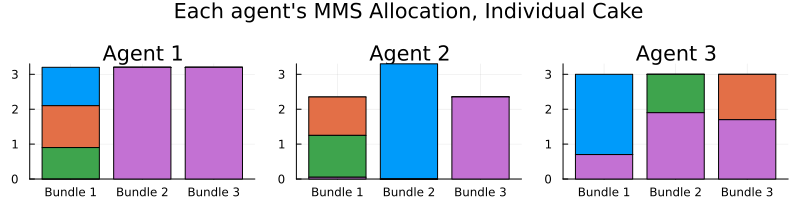
\includegraphics[width=\textwidth]{allocation_all_mms.png}
    \caption{Each Agents MMS Allocation for the individual cake instance from \autoref{subsubsec:individual-cake}.}
    \label{fig:allocation_all_mms}
\end{figure}



\subsection*{Envy-Freeness}
Envy-freeness is another common fairness notion that is prominent int the literature for indivisible goods. This project does not directly apply any of these fairness notions, but as they are still relevant i will explain them briefly here.  

\textbf{EF}\\
An allocation $\sAllocation$ is said to be envy-free (EF) if for every pair of agents $\sAgent_1,\sAgent_2 \in \sAllAgents$, we have $\sValuation_{\sAgent_1}(\sBundle_1) \geq \sValuation_{\sAgent_1}(\sBundle_2)$. In other words, no agent prefers the bundle of another agent over their own bundle.

\textbf{EF1}\\
An allocation $\sAllocation$ is said to be envy-free up to one item (EF1) if for every pair of agents $\sAgent_1,\sAgent_2 \in \sAllAgents$ there exists a good $\sGood \in \sBundle_{\sAgent_1} \cup \sBundle_{\sAgent_2}$ such that $\sValuation_{\sAgent_1}(\sBundle{\sAgent_1} \backslash \{\sGood\}) \geq \sValuation_{\sAgent_1}(\sBundle_{\sAgent_2} \backslash \{\sGood\})$. In other words, no agent prefers the bundle of another agent over their own bundle if the other agent looses one good.

\textbf{EFM}\\
An allocation $\sAllocation$ is said to satisfy \emph{Envy-Freeness for Mixed goods} (EFM) if for any agents $\sAgent_1,\sAgent_2 \in \sAllAgents$,
\begin{itemize}
    \item if agent $\sAgent_2$'s bundle consists of only indivisible goods, there exists $\sGood \in \sBundle_{\sAgent_2}$ such that $\sValuation_{\sAgent_1}(\sBundle_{\sAgent_1}) \geq \sValuation_{\sAgent_1}(\sBundle_{\sAgent_2}\backslash \{\sGood\})$;
    \item otherwise, $\sValuation_{\sAgent_1}(\sBundle_{\sAgent_1}) \geq \sValuation_{\sAgent_1}(\sBundle_{\sAgent_2})$.
\end{itemize}
Put simply, EFM is achieved if any agent that receives cake is not envied by any other agent.
From this definition we see that when the goods are all divisible, EFM reduces to EF; when goods are all indivisible, EFM reduces to EF1. Therefore EFM is a natural generalization of both EF and EF1 to the mixed goods setting.